Рассмотрим и оценим работу алгоритмов на матрицах $A[M \times N]$ и $B[N \times Q]$. 

\section{Стандартный алгоритм умножения матриц}
\qquadВ основе этого алгоритма лежит формула (\ref{formula1}). То есть для вычисления произведения двух матриц, каждая строка первой матрицы почленно умножается на каждый столбец второй, и затем подсчитывается сумма таких произведений, и полученный результат записывается в соответствующую ячейку результурующей матрицы.\\

\textbf{Схема} алгоритма представлена на Рис.\ref{fig1:image}.
\begin{figure}[h]
	\begin{center}
		{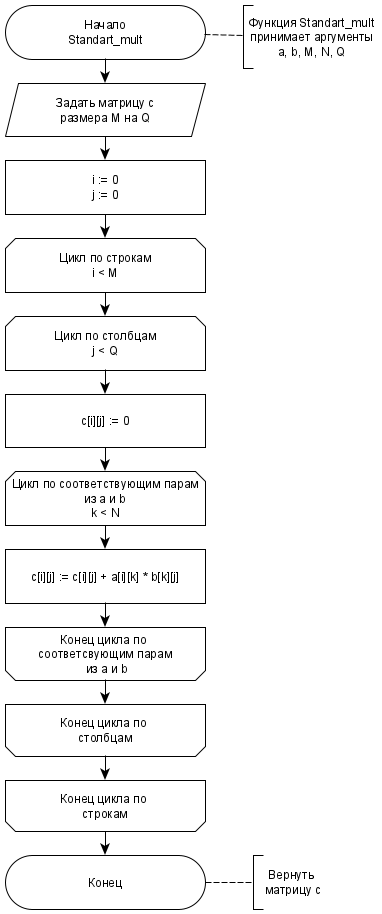
\includegraphics[scale = 0.46]{schemes/standart}}
		\caption{Стандартный алгоритм умножения матриц}
		\label{fig1:image}
	\end{center}
\end{figure}

\section{Алгоритм Винограда}
\qquadЦель данного алгоритма - сократить долю умножений в самом тяжёлом, затратном участке кода. Для этого используется формула (\ref{formula3}).\\

Некоторые из слагаемых можно вычислить заранее и использовать повторно для каждой строки первой матрицы и для каждого столбца второй. Таким образом, трудоёмкость алгоритма уменьшается за счёт сокращения количества производимых операций.\\

В этом алгоритме важно учитывать, что при нечётном значении $N$, необходимо вычислять дополнительное слагаемое $u_N \cdot v_N$.\\

\textbf{Схема} алгоритма представлена на Рис.\ref{fig2:image}.
\begin{figure}[h]
	\begin{center}
		{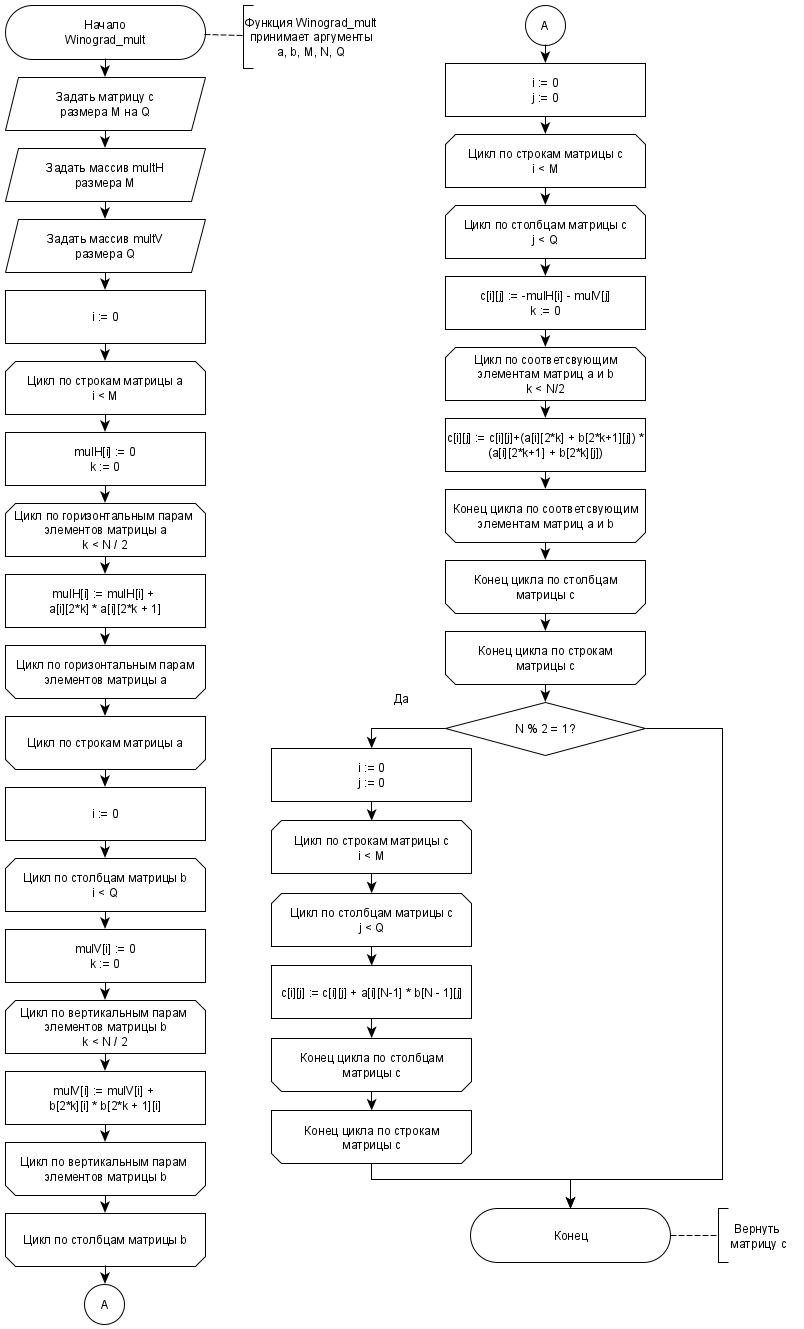
\includegraphics[scale = 0.49]{schemes/winograd}}
		\caption{Алгоритм Винограда}
		\label{fig2:image}
	\end{center}
\end{figure}

\section{Алгоритм Винограда (оптимизированный)}
\qquadАлгоритм призван уменьшить трудоёмкость алгоритма, чтобы это сделать были использованы оптимизации:
\begin{enumerate}
	\item[1)]видоизменён цикл по k, изменён шаг и условие. Таким образом, ушла необходимость в целочисленном делении, и в теле цикла не требуется больше умножать k на 2 каждый раз.
	\item[2)]введена вспомогательная переменная buf, в которую записывается промежуточнее значение соответсвующей ячейки матрицы, и затем, конечный результат переносится в саму матрицу. Тем самым, уменьшается количество обращений к элементам матрицы, находящимся по конкретному адресу.
	\item[3)]заранее высчитываются некоторые значения, например, n - 1, которые далее используюся во вложенных циклах.
	\item[4)]используется дополнительная переменная t = k - 1, чтобы сократить число подсчетов этого значения на каждом шаге цикла. 
	\item[5)]объединён цикл 3 и 4, что позволило избежать ещё одного вложенного цикла.
\end{enumerate}

\textbf{Схема} алгоритма представлена на Рис.\ref{fig3:image}.
\begin{figure}[h]
	\begin{center}
		{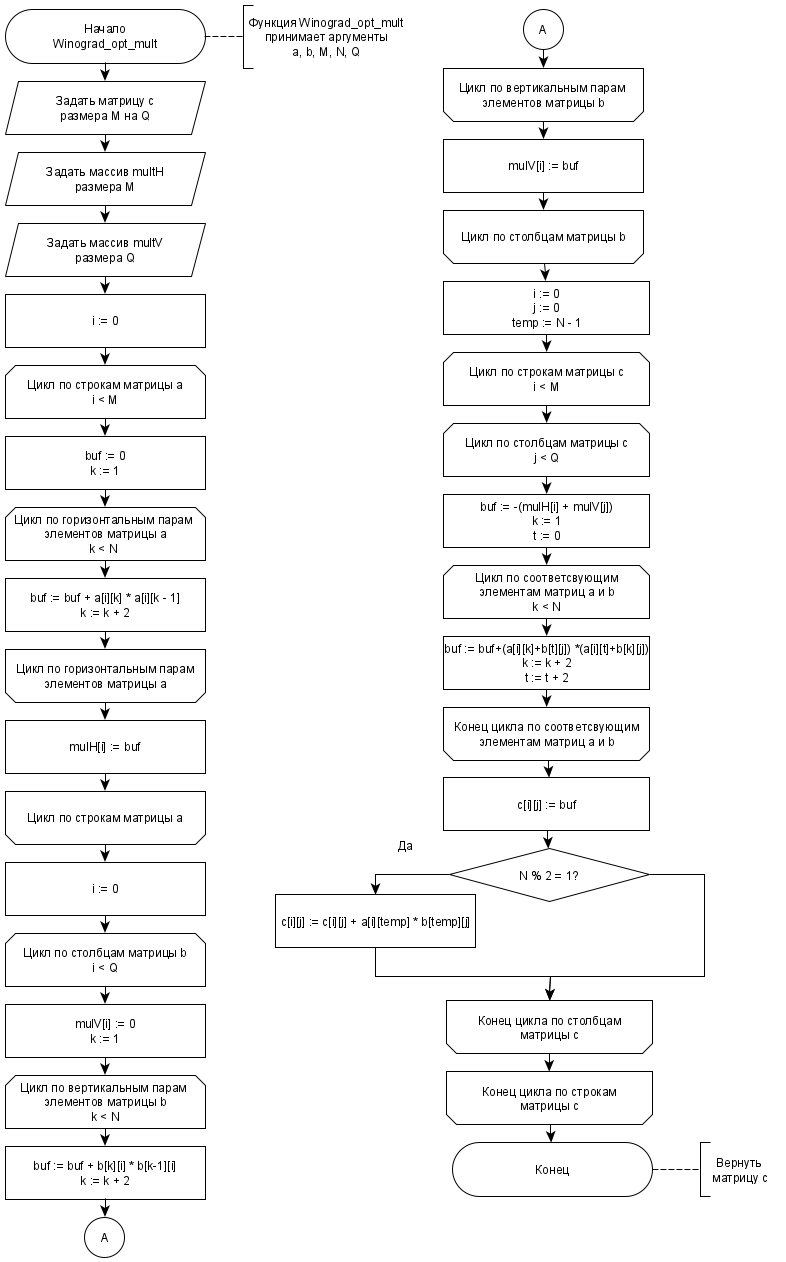
\includegraphics[scale = 0.5]{schemes/opt_winograd}}
		\caption{Оптимизированный алгоритм Винограда}
		\label{fig3:image}
	\end{center}
\end{figure}

\section{Требования к ПО}
\qquadДля корректной работы алгоритмов и проведения тестов необходимо выполнить.
\begin{enumerate}
	\item[1)]Обеспечить возможность ввода двух матриц через консоль и выбора алгоритма для умножения.
	\item[2)]Вывести, в случае ввода размеров матриц, не удовлетворяющих главному условию, соответствующее сообщение. Программа не должна аварийно завершаться.
	\item[3)]Рассчитать искомую матрицу и вывести её на экран.
	\item[4)]Реализовать функцию замера процессорного времени, которое выбранный метод затрачивает на вычисление результата. Вывести результаты замеров на экран.
\end{enumerate}


\section{Заготовки тестов}
\qquadПри проверке на корректность работы реализованных функций необходимо провести следующие тесты:
\begin{itemize}
	\item умножение матриц размером $1 \times 1$;
	\item квадратные матрицы;
	\item прямоугольные матрицы;
	\item чётное и нечётное значение $N$.
\end{itemize}